\documentclass[11pt]{article}

\usepackage[utf8]{inputenc}
\usepackage[margin=0.8in]{geometry}
\usepackage{graphicx}
\graphicspath{{img/}}
\usepackage{float}
\usepackage{amsmath}
\usepackage{amssymb}
\usepackage{setspace}
\usepackage{enumitem}
\usepackage{titlesec}
\usepackage[version=4]{mhchem}
\usepackage{siunitx}
\usepackage{comment}
\usepackage{wasysym}

\newenvironment{tight_enumerate}{
\begin{enumerate}[label=(\alph*)]
\setlength{\itemsep}{3pt}
\setlength{\parskip}{0pt}
}{\end{enumerate}}

\titleformat*{\section}{\large\bfseries}
\titleformat*{\subsection}{\normalsize\bfseries}

\title{\vspace{-3em} \textbf{Homework 1}}
\author{Justin Kang \\ AST 381: Star Formation}
\date{\vspace{-0.75em} September 19, 2018}

\begin{document}
\maketitle
\singlespacing
\pagenumbering{gobble}


\vspace{-3em}
\section*{Problem 1. Eat Your Vegetables: Radiative Transfer for the \ce{CO} Lines}
\begin{tight_enumerate}
\item Write down the steady-state rate equation describing the population of the rotational levels of \ce{CO}. Treat the radiation field by assuming that some fraction $\epsilon \leq 1$ of the photons produced following spontaneous decay, escape from the cloud containing the emitting molecules. In this approximation, the radiative term 
\[n_{k}A_{kj}+(n_{k}B_{kj}-n_{j}B_{ij})J_{\nu}\]
can be replaced by $n_{k}{\epsilon}A_{kj}.$\footnote{For the higher transitions the Einstein A coefficient can be approximated by $A_{J,J-1} = \frac{3J^{4}}{2J+1}A_{10}$. The rate coefficient can be roughly expressed as $\gamma_{J,J-1}=10^{-11}\sqrt{T}$ \si{cm^{3}s^{-1}}}.\\
\vspace{0em}\hspace{1em} The level populations are now a function of three parameters: $T$, $n(\ce{H2})$ (the collision partner density), and $\epsilon$ (the escape probability). The physical process under consideration is referred to as radiation trapping.\\
\vspace{0em}\hspace{1em} Write the population rate equation in matrix form and solve for the level populations. Check that the number of equations and the number of unknowns is sufficient to find a solution.
\item Plot level curves of the fractional level populations, $n(J)/n$, for $J = 0-5$ as a function of temperature ($0 < T < 200)$ \si{K} and \ce{H2} density ($10^{3} < n(\ce{H2}) < 10^{5}$) \si{cm^{-3}} for $\epsilon = 0.01$ and $1.0$.
\item Explain how the trapping of radiation modifies the level populations and suggests a new definition of critical density.
\item Compute the optical depth at line center for the \ce{CO} $J = 1-0$ and \ce{CO} $J = 2-1$ transitions for a typical giant molecular cloud with $A_{v} = 10$ and a \ce{CO}/\ce{H2} abundance ratio of $10^{-4}$. Assume a Doppler broadened line with a 1D velocity dispersion of $\sigma = 3\ \si{km/s}$.
\item What is the relation between $\epsilon$ and line optical depth?
\end{tight_enumerate}
\subsection*{Solution 1}
\begin{tight_enumerate}
\item We begin with the detailed balance equation for the transition between the $J = 0$ and $1$ cases, 
\[n_{0}n\gamma_{01} + n_{0}B_{01}J_{\nu} = n_{1}n\gamma_{10} + n_{1}B_{10}J_{\nu} + n_{1}A_{10}.\] 
Substituting in the radiative term, we can rearrange this equation to 
\[0 = n\gamma_{01}n_{0} - n\gamma_{10}n_{1} - {\epsilon}A_{10}n_{1}.\] 
We make the approximation $\gamma_{J,J-1} \approx \gamma_{J-1,J}$, so we can rewrite this as 
\[0 = (n\gamma_{10})n_{0} - (n\gamma_{10} + {\epsilon}A_{10})n_{1}.\]
We can now generalize this to the form 
\[0 = (n\gamma_{J+1,J})n_{J} - (n\gamma_{J+1,J} + {\epsilon}A_{J+1,J})n_{J+1}.\] 
We can easily make this into a matrix equation $A\vec{x} = \vec{0}$, where $\vec{x} = \begin{pmatrix} n_{0}, n_{1}, ..., n_{n-1}, n_{n} \end{pmatrix}^{T}$ and the $n \times (n+1)$ matrix $A$ has components $a_{i,i} = n\gamma_{J+1,J}$, $a_{i,i+1} = -(n\gamma_{J+1,J}+{\epsilon}A_{J+1,J})$, and the remaining 0. What are the dimensions of $A$? We know that $J = 0$ is the ground state of \ce{CO}, so there can be no lower level. \ce{CO} has a bond dissociation energy of 11.16 eV and the rotational energy levels are given by the equation 
\[E_{J} = \frac{\hbar^{2}}{2I}J(J+1),\] 
where $I$ is the reduced mass multiplied by the square of the bond length. The molar reduced mass of \ce{CO} is 6.86 \si{u} and the bond length of \ce{CO} is 112.8 \si{pm}. Plugging these in, we find that the maximum value of $J$ such that $E_{J}$ is less than the dissociation energy is 215. Thus we find that $A$ is a $215 \times 216$ matrix. We can notice that we need one more row in $A$ to properly solve the matrix equation. For the last row we require that each element is equal to 1, and have this row on the other side of the equation equal to 1 as well. This asserts that the level populations will sum to 1, and this way the matrix equation will solve for the specific fraction in each level population.
\item Note: the axes for these plots are in log-log scales.
\begin{figure}[H]
\vspace{-1em}
\centering
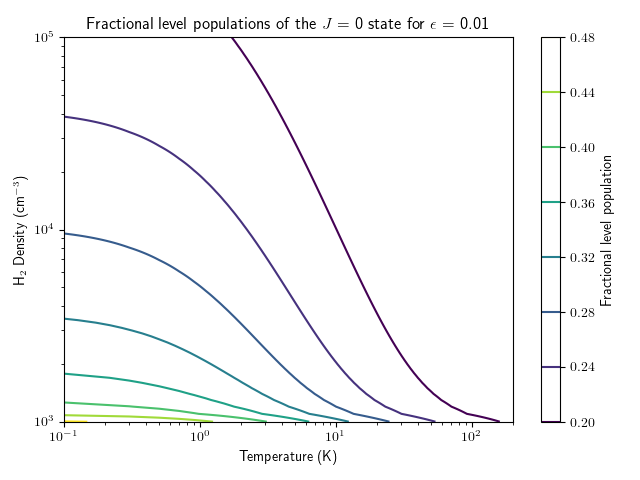
\includegraphics[height=0.25\textheight]{1/0_0.png}
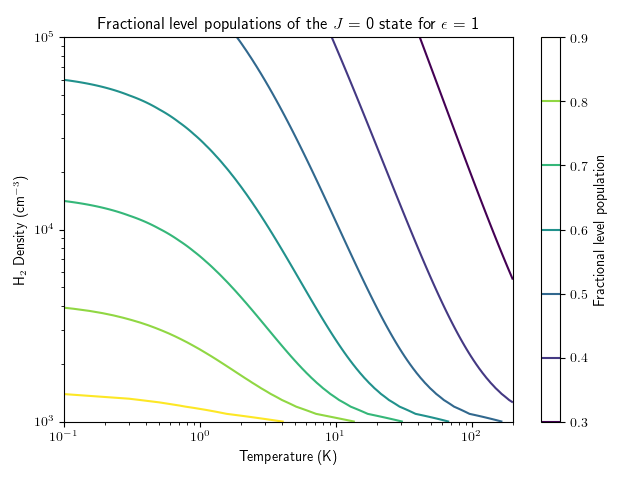
\includegraphics[height=0.25\textheight]{1/0_1.png}
\vspace{-2.5em}
\end{figure}
\begin{figure}[H]
\centering
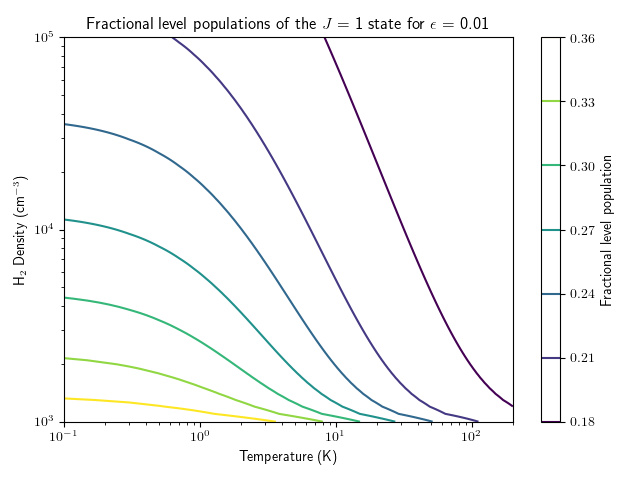
\includegraphics[height=0.25\textheight]{1/1_0.png}
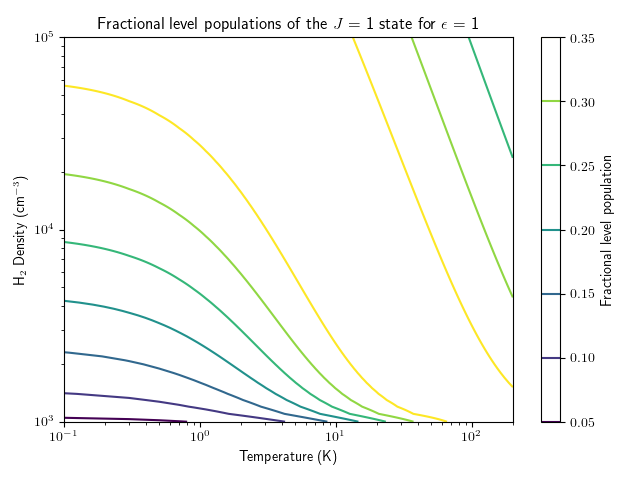
\includegraphics[height=0.25\textheight]{1/1_1.png}
\end{figure}
\begin{figure}[H]
\centering
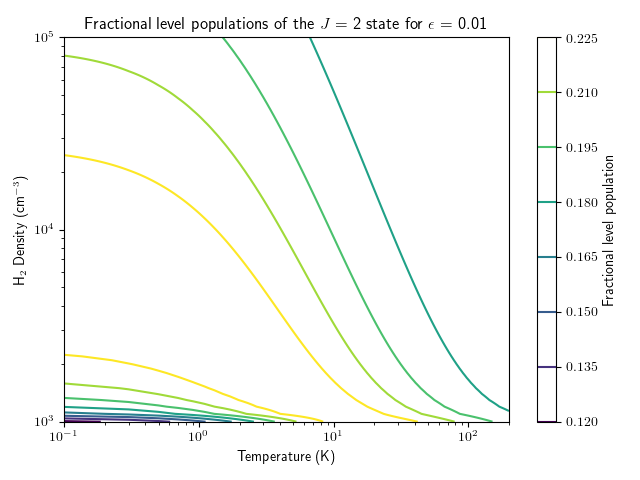
\includegraphics[height=0.25\textheight]{1/2_0.png}
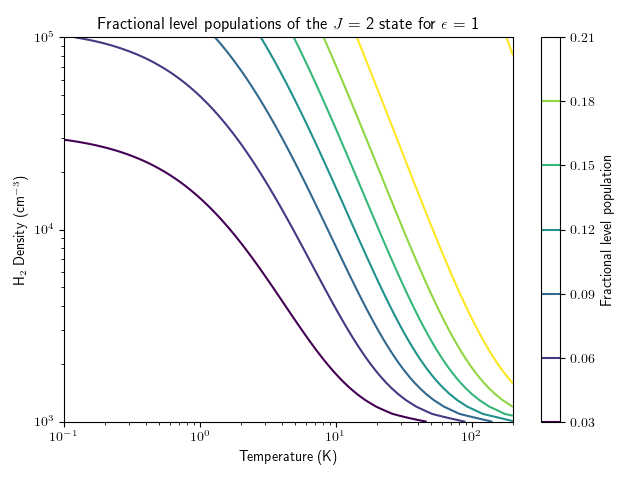
\includegraphics[height=0.25\textheight]{1/2_1.png}
\vspace{-2.5em}
\end{figure}
\begin{figure}[H]
\centering
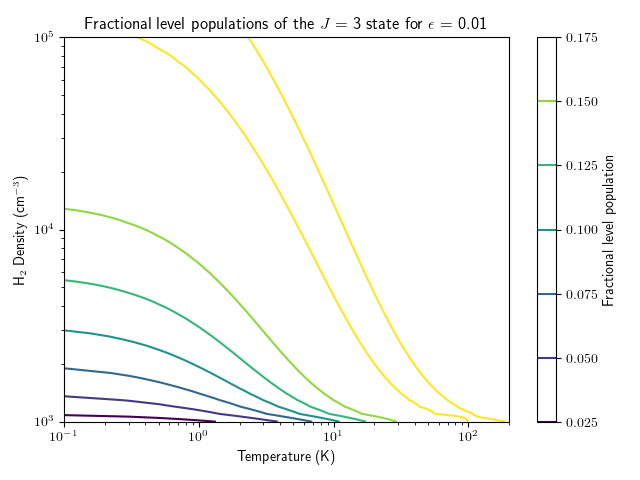
\includegraphics[height=0.25\textheight]{1/3_0.png}
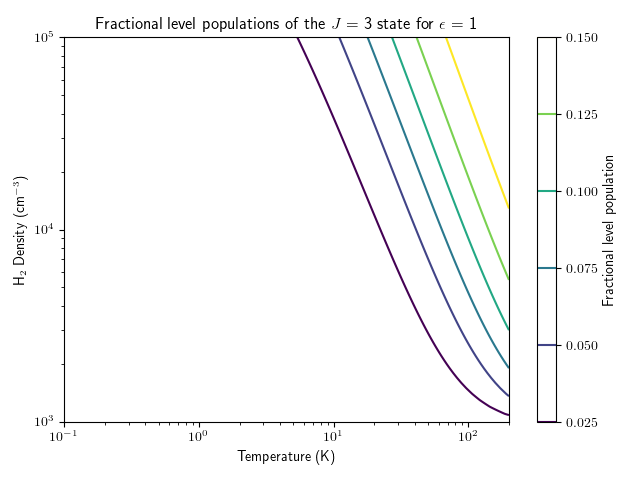
\includegraphics[height=0.25\textheight]{1/3_1.png}
\vspace{-2.5em}
\end{figure}
\begin{figure}[H]
\centering
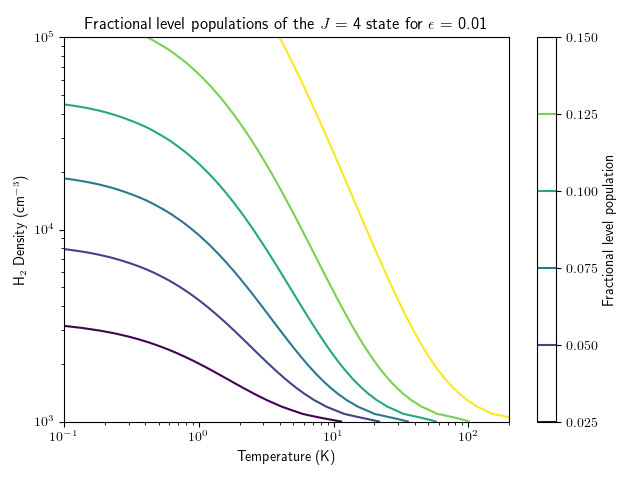
\includegraphics[height=0.25\textheight]{1/4_0.png}
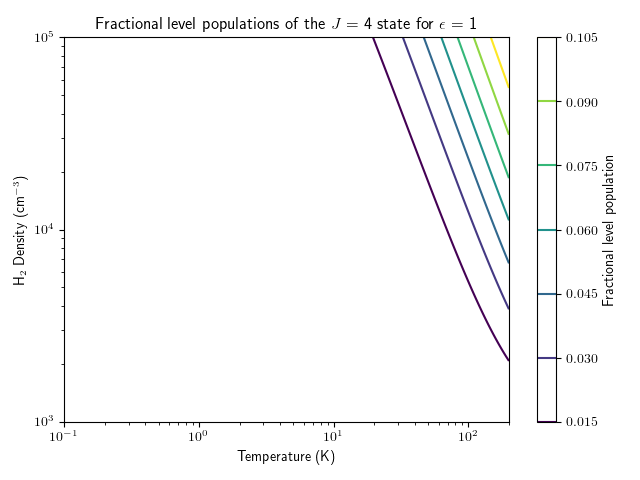
\includegraphics[height=0.25\textheight]{1/4_1.png}
\vspace{-2.5em}
\end{figure}
\begin{figure}[H]
\centering
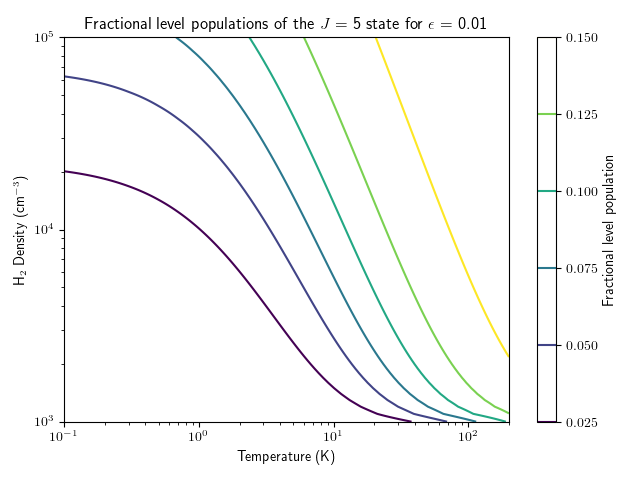
\includegraphics[height=0.25\textheight]{1/5_0.png}
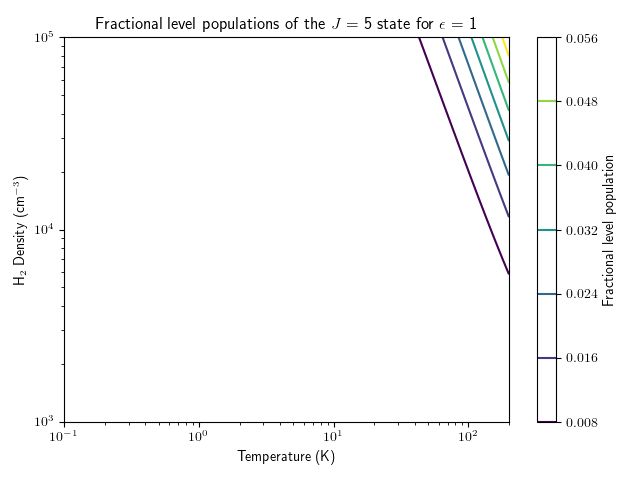
\includegraphics[height=0.25\textheight]{1/5_1.png}
\end{figure}
\item To define the critical density, we originally started with the equation 
\[n\gamma_{01}n_{0} = n\gamma_{10}n_{1} + A_{10}n_{1}\] 
and arrived at the definition $n = \frac{A_{10}}{\gamma_{01}}$. Comparing this to our substituted equation, we see that they are same minus a factor of $epsilon$ on the $A_{10}n_{1}$ term. Thus we see that radiation trapping suggests a new definition of critical density, 
\[n = \frac{{\epsilon}A_{10}}{\gamma_{01}}.\] 
Looking at the equation, this suggests that for $\epsilon < 1$ (aka radiation trapping is occurring) the critical density is lowered and thus a lower density is required for the gas to reach local thermal equilibrium. Physically, because the radiation is "trapped," the photons' energy will return to the gas (and not leave the system). As seen in the graphs, this greatly decreases both the \ce{H2} density and temperature needed to have more of the higher energy level populations.
\item The optical depth is given by the equation 
\[\tau_{ul} = \frac{A_{ul}c^{3}}{8\pi\nu_{ul}^{3}}\frac{n_{u}}{b/{\Delta}z}\left[\frac{n_{l}g_{u}}{n_{u}g_{l}}-1\right],\] 
where $b$ is the Doppler broadening parameter, ${\Delta}z$ the distance from the surface, and $g_{u}$ and $g_{l}$ the statistical weights of the upper and lower states. Given a $R_{V}$ of 3.1, we know that the hydrogen column density to visual extinction ratio is given by 
\[\frac{N(\ce{HI})+2N(\ce{H2})}{A_{v}} = 1.9 \times 10^{21}\ \si{cm^{-2}.magnitude^{-1}}.\] 
For molecular clouds, we approximate this as $\frac{N(\ce{H2})}{A_{v}} \approx 10^{21}\ \si{cm^{-2}.magnitude^{-1}}$. Using $A_{v} = 10$ we know that $N(\ce{H2}) = 10^{22}\ \si{cm^{-2}}$, and given a \ce{CO}/\ce{H2} abundance ratio of $10^{-4}$ we then know that $N(\ce{CO}) = 10^{18}\ \si{cm^{-2}}$. Now we can calculate the real (vs. fractional) number density for the upper and lower rotational levels. For the remaining variables, $A_{10} = 7.67*10^{-8}$ (Chandra et al. 1996), $\nu_{ul} = \frac{E_{u}-E_{l}}{h}$, and $g_{J} = 2J+1$. For a typical cloud, we assume $T = 10\ \si{K}$ and $n(\ce{H2}) = 300\ \si{cm^{-3}}$ (Solomon et al. 1987). We now know everything we need to calculate the optical depth. Plugging all of this in, we find that the fractional level populations for $J = 0, 1$, and $2$ are $89.97\%$, $9.90\%$, and $0.13\%$. This ultimately gives us optical depths of $459.0$ and $34.7$ for the $J=1-0$ and $J=2-1$ transitions, respectively.
\item With radiation trapping, we know that light tends to remain in the cloud, being readily reabsorbed by the gas. Because light is readily absorbed we expect a cloud with radiation trapping to be optically thick, and so trapping will lead to an increase in the optical depth. Thus the relation between $\epsilon$ and line optical depth is that they are inversely proportional.
\end{tight_enumerate}


\newpage
\section*{Problem 2. Stirring Things Up}
As we discussed in class, turbulence is often studied using numerical simulations. Data cubes of simulated density (\si{g.cm^{-3}}), and the $x$, $y$, $z$ velocity (\si{cm/s}) have been uploaded to Canvas. The simulated region has $T = 10$ \si{K} and $L = 5$ \si{pc} on a side.
\begin{tight_enumerate}
\item Plot the gas density probability distribution function (PDF). What does this suggest about the velocity dispersion? Does the simulation include gravity?
\item Use the velocity data to compute and plot the velocity power spectrum. Determine the slope, energy injection scale, and dissipation scale. What do you expect for the injection and dissipation scales for a real cloud?
\item Bonus: Given this data, do you think this is modeling a super-Alfv\'enic or sub-Alfv\'enic cloud? Why?
\end{tight_enumerate}
\subsection*{Solution 2}
\begin{tight_enumerate}
\item \leavevmode
\begin{figure}[H]
\vspace{-1em}
\centering
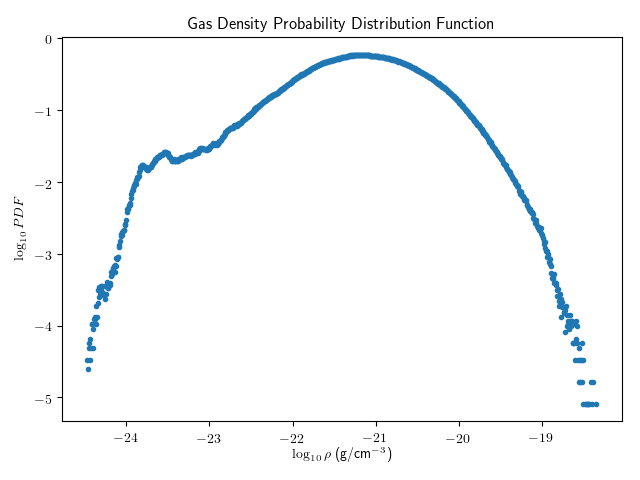
\includegraphics[height=0.4\textheight]{2/pdf.png}
\vspace{-1.5em}
\end{figure}
The probability distribution function is given by the function
\[p(\ln\rho)d\ln\rho = \frac{1}{\sqrt{2\pi\sigma^{2}}}\exp\left[-\frac{1}{2}\left(\frac{\ln\rho-\overline{\ln\rho}}{\sigma}\right)^{2}\right]d\ln\rho\]
where $\overline{\ln\rho} = -\frac{\sigma^{2}}{2}$ and $\sigma^{2} = \ln(1+b^{2}M^{2})$. The PDF is a normal distribution, thus we can numerically find the standard deviation of the distribution by using the equation 
\[\text{FWHM} = 2\sqrt{2\ln2}\sigma.\]
We then want to relate this to the Mach number $M$. Typical values of $b$ range from $0.2-0.5$, so for this case we use both to give us a range. For $b = 0.2$ $M = 3.86$, and for $b = 0.5$ $M = 1.54$. The Mach number is defined as 
\[M = \frac{u}{c_{s}},\]
where $u$ is the local flow velocity and $c_{s}$ is the sound speed. In this case we can approximate $u$ as the velocity dispersion, as we can imagine local flows like particles moving around in the cloud. This ultimately gives us a velocity dispersion of $663\ \si{m/s}$ for $b = 0.2$ and $265\ \si{m/s}$ for $b = 0.5$. 
If the simulation had gravity we would expect the edges of the PDF to flatten out, but we do not observe any such behavior in our graph. Thus the simulation doesn't include gravity.
\item \leavevmode
\begin{figure}[H]
\vspace{-1em}
\centering
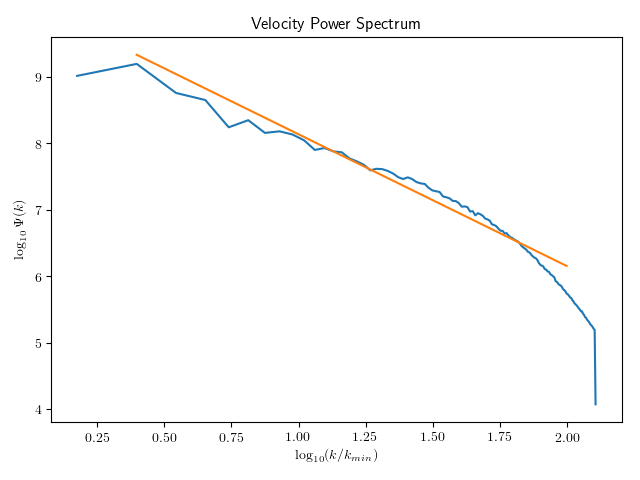
\includegraphics[height=0.4\textheight]{2/ps.png}
\vspace{-1.5em}
\end{figure}
The power spectrum is given by the function 
\[\mathbf{\Psi(x)} = |\mathbf{v(k)}|^{2},\]
where $\mathbf{v(k)} = \frac{1}{(2\pi)^{3/2}}\int{\mathbf{v(x)}e^{-i\mathbf{k \cdot x}}}$. To plot this we simply read in the data, apply a FFT on it to get from physical to phase space, and then produce the power spectrum. The code to generate this power spectrum closely follows the template provided by the yt Project\footnote{http://yt-project.org/doc/cookbook/calculating\_information.html}. Because we know from a) that the Mach number of the gas is greater than 1, we expect the fluid to be in the compressible regime (and thus have a slope in the inertial region of -2). By fitting the linear regime of the graph, we find that it has a slope of $-1.984\pm0.045$, which is within error of the $-2$ that we expect. For the energy injection and disspitation scales, we find the values of $k$ such that $\mathbf{\Psi(k)}$ is turning over in the graph. These $k$ values are $2.269*10^{-19}$ and $5.801*10^{-18}$, respectively. Converting this back into spatial dimensions using $k = \frac{2\pi}{L}$, we find that the corresponding length scales are $8.976\ \si{pc}$ for the energy injection scale and $0.351\ \si{pc}$ for the dissipation scale. If we choose to follow Kolmogorov turbulence as representative of real clouds, we'd expect the injection scale to be on the order of the cloud size ($\approx 10\ \si{pc}$) and the dissipation scale to be small ($<\ \si{AU}$). Thus we find that our numbers agree with the injection scale, but are several orders of magnitude above the dissipation scale. This is possibly due to the fact that we're working with a compressible fluid, rather than the incompressible one Kolmogorov assumed for his analysis.
\item \frownie
\end{tight_enumerate}


\newpage
\section*{Problem 3. Mystery Region}
A \ce{^{12}CO} (1-0) data cube of a mystery region has been uploaded to Canvas. Use what you've learned so far about \ce{CO}, turbulence, and clouds to figure out some information about this region: Is this cloud star-forming? What is the cloud velocity dispersion and Mach number? Is it a "low-mass" or "high-mass" region? Justify your answers.
\subsection*{Solution 3}
One of the dimensions provided in the mystery FITS file is dimension, which spans 301 cells and physically ranges between $-1$ to $3\ \si{km/s}$. Visualizing the velocity in DS9, we find that at a velocity of $6\ \si{km/s}$, we find that there is a bimodal distribution in the velocity profile. This is indicative of feedback, which suggests that there are high-mass stars in the region. Thus we expect the cloud to be star-forming. Taking the standard deviation over all of the velocity axis to roughly be the velocity dispersion, we find that that cloud velocity dispersion is $11.585\ \si{km/s}$. Assuming typical cloud conditions ($T = 10\ \si{K}$), the Mach number is then $M = \frac{\sigma}{c_{s}} = 0.06749$. Because $M \ll 1$, we see that this is a highly subsonic region. If we suppose that the cloud is in virial equilibrium we can find the virial mass, which would serve as a good estimator for the true mass. Assuming the cloud is spherical we can use the equation $\frac{3}{5}\frac{GM}{R} = \frac{1}{2}\sigma^{2}$. Typical molecular clouds have sizes on the order of $10\ \si{pc}$; using this for $R$, we find that the virial mass is around $2.6*10^{5}\ M_{\odot}$. Most clouds tend to have a virial paramter $\alpha > 2$, we can expect this to be an overestimate of the true mass. Given that molecular clouds have a mass range of about $10^{4}-10^{7}\ M_{\odot}$, we expect this to be a "low-mass" region. 
% TODO: is the cloud star-forming?
% visually inspect and do 3d profile to see velocities -> velocity dispersion -> feedback (double peak velocity profile) -> high mass stars


\end{document}